\chapter{Testing for Trend in Dose-response Microarray Experiments}
\markchapter{Testing for Trend in Dose-response Microarray
Experiments} \label{chap: testfortrend}

\section{Testing for Homogeneity of the Means Under Restricted
Alternatives} \label{sec: testing}

In this section, we review several procedures for testing the
homogeneity of the means against order restricted alternatives. In
particular we focus on four existing procedures: Williams' (Williams
1971 and 1972), Marcus' (Marcus 1976), the global likelihood ratio
test (Bartholomew 1961, Barlow \textit{et al.}\ 1972, and Robertson
\textit{et al.}\ 1988), and the $M$ (Hu \textit{et al.}\ 2005)
statistic. Additionally, we introduce a modification to the degrees
of freedom of the $M$ statistic.
%\subsection {\textbf{Test of Homogeneity of the Means Under Restricted
%Alternatives}}

In the microarray experiment, for each gene, the following ANOVA
model is considered:
\begin{equation}
\label{themodel} Y_{ij}=\mu(d_{i})+\varepsilon_{ij},\;i=0,1,\dots,
K,\;j=1,2, \dots, n_i,
\end{equation}
where $Y_{ij}$ is the $j$th gene-expression at the \textit{i}th dose
level, $d_{i}$ ($i=0,1,\dots, K$) are the \textbf{$K$+1} dose
levels, $\mu(d_{i})$ is the mean gene-expression at each dose level,
and $\varepsilon_{ij} \sim N(0,\sigma^{2})$.

The null hypothesis of no dose effect is given by
\begin{equation}
\label{null}
\begin{array}{l}
H_{0}:\mu(d_{0})=\mu(d_{1})= \dots =\mu(d_{K}).
\end{array}
\end{equation}
A one-sided alternative hypothesis of a positive dose effect for at
least one dose level (i.e., an increasing trend) is specified by
\begin{equation}
\label{h1up} H^{Up}_{1}: \mu(d_{0}) \le \mu(d_{1}) \le \cdots \le
\mu(d_{K}),
\end{equation}
with at least one strict inequality. When testing the effect of a
drug for a positive outcome the researcher can specify a positive
effect as the desirable alternative. However, in the current
microarray setting, it seems reasonable to assume that the
gene-expression levels may increase or decrease in response to
increasing doses, but with the direction of the trend not known in
advance. Thus, we must also consider an additional alternative:
\begin{equation}
\label{h1down} H^{Down}_{1}: \mu(d_{0}) \ge \mu(d_{1}) \ge \cdots
\ge \mu(d_{K}),
\end{equation}
with at least one strict inequality.
%To be complete, the general unrestricted alternative hypothesis of
%\begin{equation}
%\label{h1neq}
%\begin{array}{l}
%H_{2}: \mu(d_{0}) \neq \mu(d_{1}) \neq \cdots \neq \mu(d_{K}),\\
%\end{array}
%\end{equation}
%can be considered as well.
%In what follows we focus on testing $H_1$ versus $H_0$,
%although we briefly discuss the testing procedure of $H_2$ versus $H_1$ (\citealp{Bartholomew} 1961) in
%Section 3.3.
Testing $H_{0}$ against $H^{Down}_{1}$ or $H^{Up}_{1}$ requires
estimation of the means under both the null and the alternative
hypotheses. Under the null hypothesis, the estimator for the mean
response $\hat{\mu}$ is the sample mean. Let
$\hat{\mu}^{\star}_{0},\hat{\mu}^{\star}_{1},\dots,\hat{\mu}^{\star}_{K}$
be the maximum likelihood estimates for the means (at each dose
level) under the ordered alternative. Barlow \textit{et al.}~(1972)
and Robertson \textit{et al.}~(1998) showed that
$\hat{\mu}^{\star}_{0},\hat{\mu}^{\star}_{1},\dots,\hat{\mu}^{\star}_{K}$
are given by the isotonic regression of the observed means.

%In what follows, we briefly describe the tests we consider.

\subsection{Williams' (1971, 1972) and Marcus' (1976) Test Statistics}

Williams' procedure defines $H_{0}$ as the null hypothesis, and
$H_{1}^{Up}$ or $H_{1}^{Down}$ as the one-sided alternative.
Williams' (1971, 1972) test statistic was suggested for a setting,
in which $n_{i}$ observations are available at each dose level. As
all dose levels are compared with the control level, the test
statistic is given by
\begin{equation}
\label{wil1} t_{i}=\frac{\hat{\mu}^{\star}_{i}-\bar{y}_{0}}{\sqrt{2
s^{2}/r}}.
\end{equation}
Here, $\bar{y}_{0}$ is the sample mean at the first dose level
(control), $\hat{\mu}_{i}^{\star}$ is the estimate for the mean at
the $i$th dose level under the ordered alternative, $r$ is the
number of replications at each dose level, and $s^{2}$ is an
estimate of the variance. For $\hat{\mu}_{i}^{\star}$, Williams
(1971, 1972) used the isotonic regression of the observed response
with respect to dose (Barlow \textit{et al.}\ 1972). Williams' test
procedure is a sequential procedure. In the first step,
$\hat{\mu}_{K}^{\star}$ is compared to $\bar{y}_{0}$. If the null
hypothesis is rejected, $\hat{\mu}_{K-1}^{\star}$ is compared to
$\bar{y}_{0}$, etc.

Marcus (1976) proposed a modification to Williams' test statistic
that replaced $\bar{y}_{0}$ with $\hat{\mu}_{0}^{\star}$, the
estimate of the first dose (control) mean under ordered restriction.
Marcus' test statistic performs closely to Williams' in terms of
power (Marcus 1976). Note that, for $K=1$, Williams' and Marcus'
test statistics reduce to the two-sample t-test.


\subsection{Likelihood Ratio Test Statistic for Monotonicity\\
(Barlow \textit{et al.}\ 1972, and Robertson \textit{et al.}\ 1988)}

Williams' and Marcus' procedures are step-down procedures, i.e., the
comparison between a lower dose and control is tested only if the
test of a higher dose vs.\ control is significant. The underlying
assumption is that there is a monotone dose-response relationship
with a known direction.

%i.e., for $k$ dose levels it is assumed that $\mu_{0} \le
%\mu_{1} \le \dots \le \mu_{k}$.
Testing the equality of ordered means using likelihood ratio tests
(when response is assumed to be normally distributed) was discussed
by Barlow \textit{et al.}\ (1972) and Robertson \textit{et al.}\
(1988). Both authors considered the likelihood ratio test, in which
the variance under the null and the alternative were compared.
%\citealp{Barlow} (1972) and
%\citealp{Robertson} (1988) showed that
%$\hat{\mu}^{\star}_{0},\hat{\mu}^{\star}_{1},\hat{\mu}^{\star}_{2},\hat{\mu}^{\star}_{3}$
%are mean estimates from the isotonic regression.
The likelihood ratio test statistic is given by
\begin{equation}
\label{lr1}
\Lambda_{01}^{\frac{2}{N}}=\frac{\hat{\sigma}^{2}_{H_{1}}}{\hat{\sigma}^{2}_{H_{0}}}=\frac{\sum_{ij}
(y_{ij}-\hat{\mu}^{\star}_{j})^{2}}{\sum_{ij}(y_{ij}-\hat{\mu})^{2}},
\end{equation}
where $\hat{\sigma}^{2}_{H_{0}}$ and $\hat{\sigma}^{2}_{H_{1}}$ are
the estimates for the variance under the null and the alternative
hypothesis, respectively. And $\hat{\mu}=\sum_{ij}y_{ij}/\sum_i n_i$
is the overall mean. The null hypothesis is rejected for a ``small"
value of $\Lambda_{01}^{\frac{2}{N}}$. Equivalently, $H_{0}$ is
rejected for large value of $\bar{E}^{2}_{01}$, where
\begin{equation}
\bar{E}^{2}_{01}=1-\Lambda^{\frac{2}{N}}_{01}=
\frac{\sum_{ij}(y_{ij}-\hat{\mu})^{2}-\sum_{ij}
(y_{ij}-\hat{\mu}^{\star}_{j})^{2}}{\sum_{ij}(y_{ij}-\hat{\mu})^{2}}.
\label{lr2}
\end{equation}
Estimating the parameters using isotonic regression requires the
knowledge of the direction of the trend. In practice, the direction
of the trend is often not known in advance. In such a case one can
maximize the likelihood twice: for a monotone decreasing trend and
for a monotone increasing trend, and choose the trend with a higher
likelihood. In practice, we can calculate $\bar{E}^{2}_{01}$ for
each direction and choose the higher value of $\bar{E}^{2}_{01}$
(Barlow \textit{et al.}\ 1972). A resampling-based approach, as
described in Section 3.2.2, can be used to approximate the null
distribution for the test statistic, so that two-sided $p$-values
are obtained for inference.



\subsection{{The $M$ Test Statistic of Hu \textit{et al.}} (2005)}

Recently, Hu \textit{et al.}\ (2005) proposed the following test
statistic $M$ to test for a monotonic trend:
\begin{equation}
\label{Mstat}
M=\frac{\hat{\mu}^{\star}_{K}-\hat{\mu}^{\star}_{0}}{\sqrt{\sum_{i=0}^{K}
\sum_{j=1}^{n_{i}} (y_{ij}-\hat{\mu}^{\star}_{i})^2/(n-K)} }.
\end{equation}
where $n$ is the total number of arrays.

Hu \textit{et al.}\ (2005) discussed a setting, in which the
comparison of primary interest is the difference between the highest
dose level $(K)$ and the control dose. The numerator of the $M$ test
statistic is the same as that of Marcus' statistic, while the
denominator is an estimate of the standard error under an ordered
alternative. This is in contrast to Williams' and Marcus' approaches
that use the unrestricted means to derive the estimate for the
standard error.

Hu \textit{et al.}\ (2005) evaluated the performance of the
$\bar{E}^{2}_{01}$ and $M$ test statistics by comparing the ranks of
genes obtained by using both statistics, and reported similar
findings for simulated and real-life data sets.

\subsection{A Modification to the $M$ Test Statistic (Lin \textit{et al.}~2007)}
For the variance estimate, Hu \textit{et al.}\ (2005) used $n-K$
degrees of freedom (see equation~(\ref{Mstat})). However, the unique
number of isotonic means is not fixed, but changes across the genes.
For that reason, we propose a modification to the standard error
estimator used in the $M$ statistic by replacing it with
$\sqrt{\sum_{i=0}^{K} \sum_{j=1}^{n_{i}}
(y_{ij}-\hat{\mu}^{\star}_{i})^2/(n-I)}$, where $I$ is the unique
number of isotonic means for a given gene. Such a modification is
expected to improve the standard error estimates across all the
genes.

The five test statistics are implemented in the $R$ \texttt{IsoGene}
package, which is discussed in detail in the next chapter.

%Details on functions in the package are discussed in Chapter 9.


%The performance of the three estimators of the standard errors
%discussed above is compared in a simulation study which we discuss
%in Section 6.

\section{Directional Inference }
\label{sec: directional/multiplicity}



\subsection{{Directional Inference in Isotonic Regression}}
\label{sec: directional}

%As the four test statistics discussed above, they are one sided test statistics.
The five test statistics discussed in Section~\ref{sec: testing}
should be calculated assuming a particular direction of the ordered
alternative. However, the direction of the test is unknown in
advance. In this section, we address the issue of how to obtain the
two-sided $p$-value from the five testing procedures, and how to
determine the direction of the trend from two-sided $p$-value
afterwards.

%Especially we discuss the property of the statistics for directional
%inference in detail.

We focus on the two possible directions of the alternatives:
$H^{Up}_{1}$ defined in equation (3) and $H^{Down}_{1}$ defined in
equation (4). Let $p^{Up}$ and $T^{Up}$ denote the $p$-value and the
corresponding test statistic computed to test $H_0$ vs.\
$H^{Up}_{1}$, and let $p^{Down}$ and $T^{Down}$ denote the $p$-value
and the corresponding test statistic computed to test $H_0$ vs.\
$H^{Down}_{1}$. Barlow \textit{et al.}\ (1972) showed that, for
$K>2$, a $\bar{\chi}^2$ statistic for testing $H_0$ may actually
yield $p^{Up} < \alpha$ and $p^{Down} < \alpha$. However, $p = 2
\min (p^{Up}, p^{Down})$ is always a conservative $p$-value for the
two-sided test of $H_0$ vs.\ either $H^{Up}_1$ or $H^{Down}_1$.

Hu \textit{et al.}\ (2005) adapted the approach by taking the larger
of the likelihoods of $H^{Up}_{1}$ or $H^{Down}_{1}$, i.e., the
larger of $T^{Up}$ and $T^{Down}$ is used as the test statistic for
the two-sided inference. In contrast to Hu \textit{et al.}\ (2005),
we obtain two-sided $p$-values by taking $p = \min( 2 \min (p^{Up},
p^{Down}), 1)$, where $p^{Up}$ and $p^{Down}$ are calculated for
$T^{Up}$ and $T^{Down}$ using permutations to approximate the null
distribution of these test statistics. We use $p^{Up}$ and
$p^{Down}$ to determine the direction of the trend, as described
below.

After rejecting the null hypothesis against the two-sided test there
is still a need to determine the direction of the trend. The
direction can be inferred by the following procedure. If $p^{Up} \le
\alpha/2$, then reject $H_0$ and declare $H_1^{Up}$; if $p^{Down}
\le \alpha/2$, then reject $H_0$ and declare $H_1^{Down}$. The
validity of this directional inference is based on the following
property: under $H^{Up}_{1}$, $p^{Down}$ is stochastically larger
than $U[0,1]$; and under $H^{Down}_{1}$, $p^{Up}$ is stochastically
larger than $U[0,1]$ (proof not given here). Thus, the probability of falsely rejecting
$H_0$ is $\le \alpha$, and the probability of declaring a wrong
direction for the trend is $\le \alpha/2$. It is also important to
note that the event $p^{Up} < \alpha/2$ and $p^{Down} < \alpha/2$
may be observed. Under $H_0$, $H^{Up}_{1}$, or $H^{Down}_{1}$, this
event is unlikely. However, it is likely if the treatment has a
large and non-monotone effect.  

%An example of this unique situation,
%in which the null hypothesis can be rejected for both directions, is
%given in Section~\ref{sec: genes}.

%%change the sentense here

In order to illustrate whether the property needed for directional
inference applies to the five test statistics, we conduct a
simulation study to investigate the distribution of the $p^{Up}$ and
$p^{Down}$ values. For each simulation, data are generated under
$H_1^{Up}$: the means are assumed to be equal to $(1,\; 2, \;3, \;4)
/\sqrt{5}$ for the four doses, respectively, and the variance is
equal to $\sigma^2=1$. The test statistics $T^{Up}$ and $T^{Down}$
are calculated for the two possible alternatives $H_1^{Up}$ and
$H_1^{Down}$. Their corresponding $p^{Up}$- and $p^{Down}$-values
are obtained using 10,000 permutations.

Figure~\ref{pupdn1} shows the cumulative distribution of $p^{Up}$
and $p^{Down}$. Clearly, the simulations show that the cumulative
distribution of $p^{Down}$ (the $p$-value of the test statistics
calculated assuming the wrong direction, dotted line in
Figure~\ref{pupdn1}) is stochastically higher than $U[0,1]$ (solid
line in Figure~\ref{pupdn1}), which is the distribution of the
$p$-values under the null hypothesis. Moreover, the distribution of
$p^{Up}$ (the $p$-value for the test statistics calculated assuming
the right direction, dashed line in Figure~\ref{pupdn1}) is, as
expected, stochastically smaller than $U([0,1]$. Similar results
(not shown) are obtained when the data are generated under
$H_{1}^{Down}$. The results imply that all the five test statistics
possess the property required for the directional inference: under
$H^{Up}_1$ the distribution of $p^{Down}$ is stochastically greater
than $U[0,1]$.

%\begin{center}
%Figure~\ref{pupdn1}-ABOUT HERE
%\end{center}


\begin{figure}[!h]
\centering
{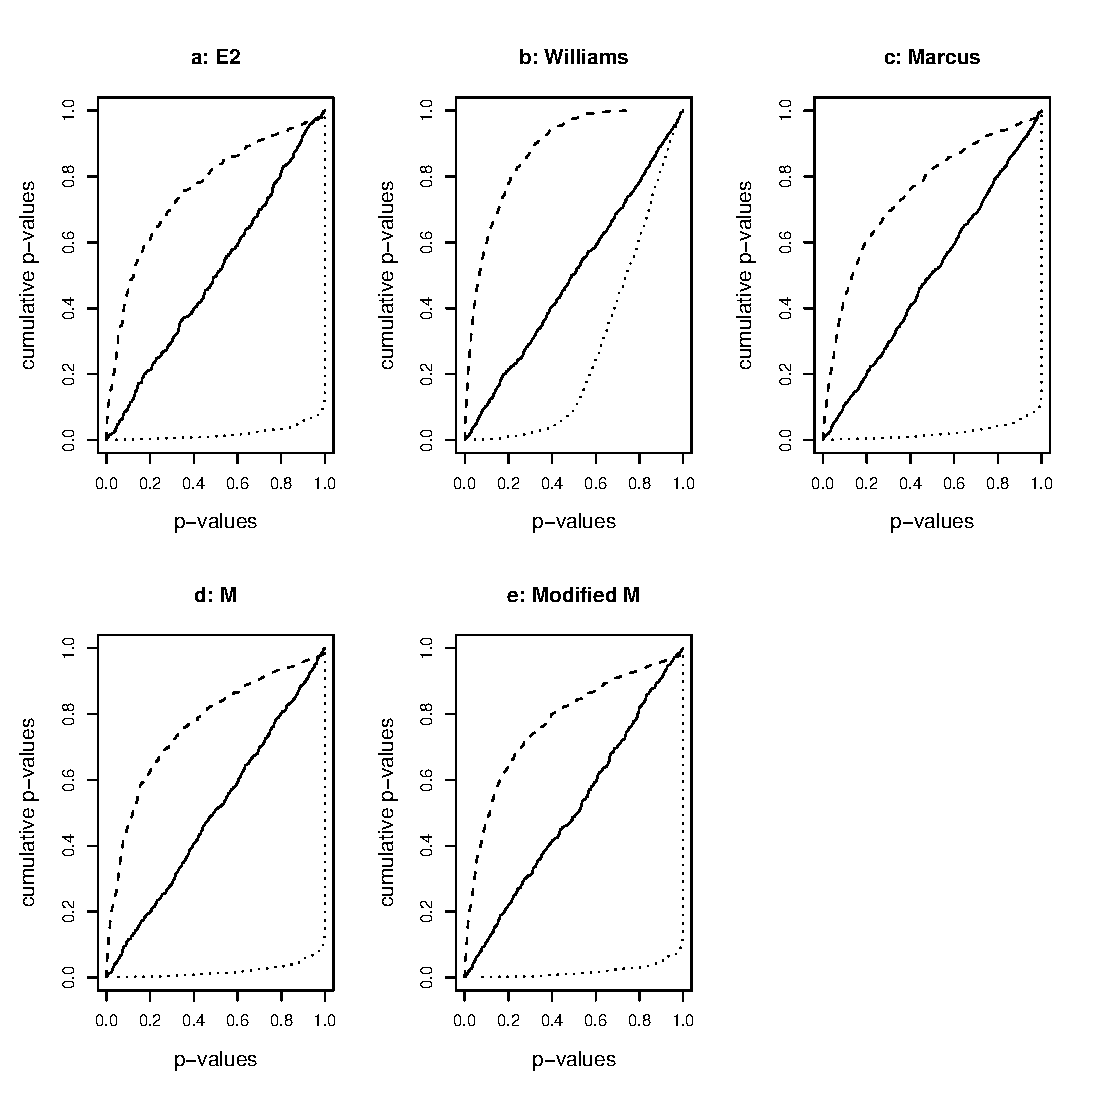
\includegraphics[width=.9\textwidth]{pupdn1b.eps}}
\caption{\em{The cumulative distribution of $p^{Up}$-values (dashed
line) and $p^{Down}$-values (dotted line) for the five test
statistics. Data are generated under $H_1^{Up}$ with isotonic means
(1, 2, 3, 4)/$\sqrt{5}$ for the four doses. Solid line: cumulative
distribution of $H_0\sim U[0,1]$.}} \label{pupdn1}
\end{figure}


Figure~\ref{stat1} shows the values of test statistics, which were
calculated under $H^{Up}_1$ and $H^{Down}_1$, for data generated
under $H^{Up}_1$. The five test statistics are calculated for
testing $H_0$ vs.\ $H^{Down}_1$ (the x-axis of each test statistic
in Figure~\ref{stat1}). The behavior of Marcus', $M$, and the
modified $M$ statistics is similar as they all use the difference
between the highest and the lowest isotonic mean.
%Marcus', $M$ and the modified $M$ test always forces the estimated trend to be decreasing or flat.
The maximum value of the test statistics (when calculated assuming
the wrong direction) is equal to zero. In contrast, Williams' test
statistic for testing $H_0$ vs.\ $H^{Down}_1$ (shown on the x-axis
of the panel $b$) can be positive or negative, because the sample
mean of control group is used instead of the isotonic mean. Note
that we reject the null hypothesis in favor of $H^{Down}_1$ for
negative values of the test statistic. Further, the value of the
test statistics for testing $H_0$ vs.\ $H^{Up}_1$ (the y-axis of
Figure~\ref{stat1}) is higher than the value of the test statistics
calculated for testing $H_0$ vs.\ $H^{Down}_1$ (the x-axis of
Figure~\ref{stat1}).



\begin{figure}[!h]
\centering
{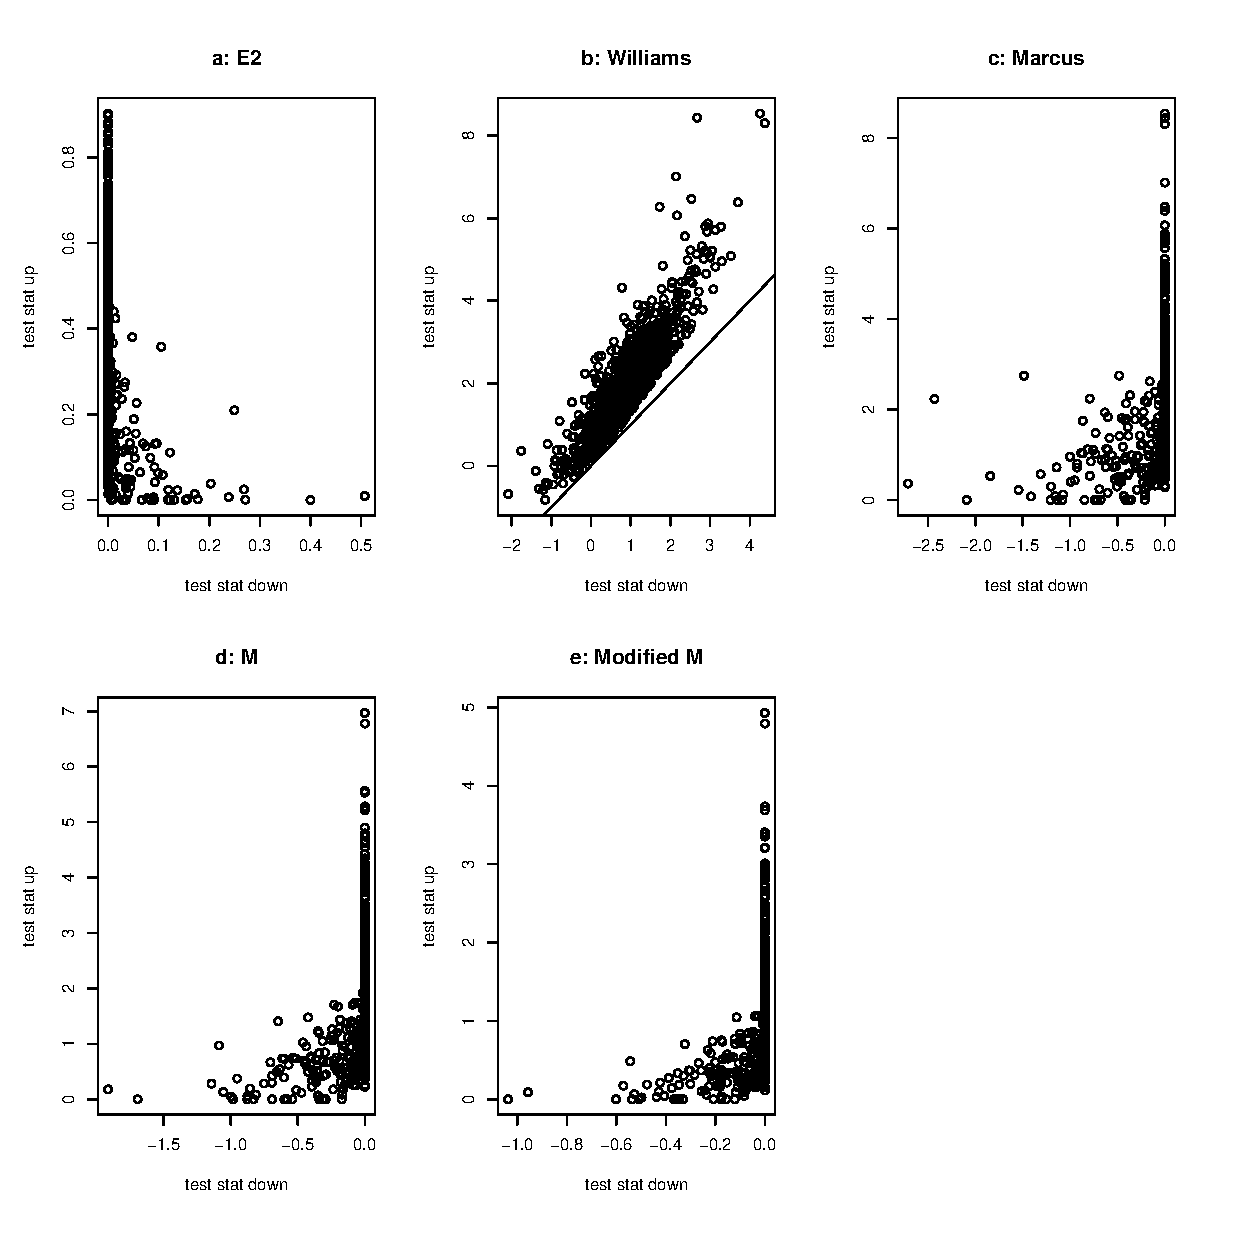
\includegraphics[width=.9\textwidth]{stat1a.eps}}
\caption{\em{The five test statistics calculated for $H_0$ vs.\
$H_1^{Up}$ (y-axis) and $H_0$ vs.\ $H_1^{Down}$ (x-axis).}}
\label{stat1}
\end{figure}








\subsection{Control of the Directional FDR}
\label{sec: FDR}

When the FDR controlling procedures are used to adjust for multiple
testing in the microarray setting, the set of two-sided $p$-values
computed for each gene is adjusted by using the BH-FDR or BY-FDR
procedure described in Section 3.2.1. A discovery in this case is a
rejection of $H_0$ for some gene; a false discovery is to reject
$H_0$ when $H_0$ is true. As mentioned before, in a microarray
dose-response experiment we are also interested in the direction of
the dose-response trend.

Benjamini and Yekutieli (2005)
% reference:
% \bibitem{BY} Benjamini Y., Yekutieli D., (2005a)
% ``False Discovery Rate-Adjusted Multiple Confidence Intervals for Selected Parameters''
% {\em Journal of the American Statistical Association}, {\bf 100}, 71-81.
provide a framework for addressing the multiplicity problem when
attempting to determine the direction of multiple parameters: a
discovery is to declare the sign of a parameter as either being
positive or negative. Three types of false discoveries are possible:
declaring a zero parameter either as negative or as positive,
declaring a negative parameter as positive, and declaring a positive
parameter as negative. The FDR corresponding to these discoveries is
termed the Mixed Directional FDR (MD-FDR). In the current setting,
the MD-FDR is the expected value of the number of genes, for which
$H_0$ is true, that are erroneously declared to have either a
positive or negative trend plus the genes with a monotone trend but
with a wrong direction of the declared trend, divided by the total
number of genes declared to have a trend. Benjamini and Yekutieli
(2005) prove that if $p$-values pose the directional property
described in Section~\ref{sec: directional}, then applying the BH
procedure at level $q$ to the the set of two-sided $p$-values
computed for each gene, and declaring the direction of the trend
corresponding to the smaller one-sided $p$-value, controls the
MD-FDR at level $q/2 \cdot (1 + m_0/m)$, where $m$ is the total
number of genes and $m_0$ is the number of genes, for which $H_0$
holds.

In general, directional inference is a more general setting than
hypotheses testing (Benjamini and Yekutieli, 2005). Nevertheless, as
a false discovery is made based on the $p$-value that is
stochastically larger than $U[0,1]$, then the resampling-based
methods that control the FDR (Yekutieli and Benjamini, 1999) also
control the MD-FDR. This is achieved by simply applying the
resampling-based procedure to test $H_0$, and if $H_0$ is rejected,
declaring the direction of the trend according to the minimum
one-sided $p$-value. For each rejected null hypothesis it is also
advisable to examine if the larger $p$-value is $\le \alpha$. If
this is the case, this may serve as an indication of a non-monotone
dose-response relationship.

